\subsection{Kinematic Model Calculation}
The three-wheeled mobile robot is used in other two papers \cite{three_wheel} \cite{motion_control} however, they do not provide the procedure to compute its kinematic model, therefore for completeness we show here the steps necessary to obtain (\ref{eq:kin_model}). The initial steps are similar to the proof shown in \cite{proof_model}.

The type of onmi-wheel used by the robot is shown in Fig.\ref{fig:omniwheel}, please notice axes of rollers are perpendicular ($90^{\circ}$) to the wheel axis, we made this clarification to avoid confusion with Mecanum wheel (a.k.a. Swedish wheel) in which axes of rollers have an angle of $45^{\circ}$, this last type is usually used in four-wheeled robot.
\begin{figure}[h]
    \centering
    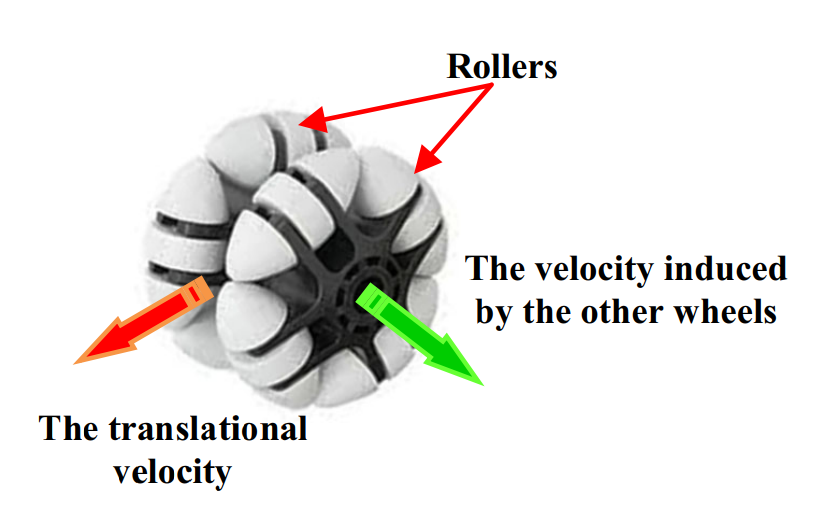
\includegraphics
        [width=0.4\textwidth]
        {figures/omniwheel.png}
    \caption{Omnidirectional wheel mounted on three-wheeled robot. Credit: \cite{proof_model}}
    \label{fig:omniwheel}
\end{figure}    
    
The first step is to compute the velocity induced to other wheels when a wheel rotates around its axis. Once computed it we can easily obtain the kinematic model w.r.t. to the robot's coordinate system $RF_m$ and then w.r.t. $RF_w$. 

\subsubsection{Induced velocity}
\begin{figure}[h]
    \centering
    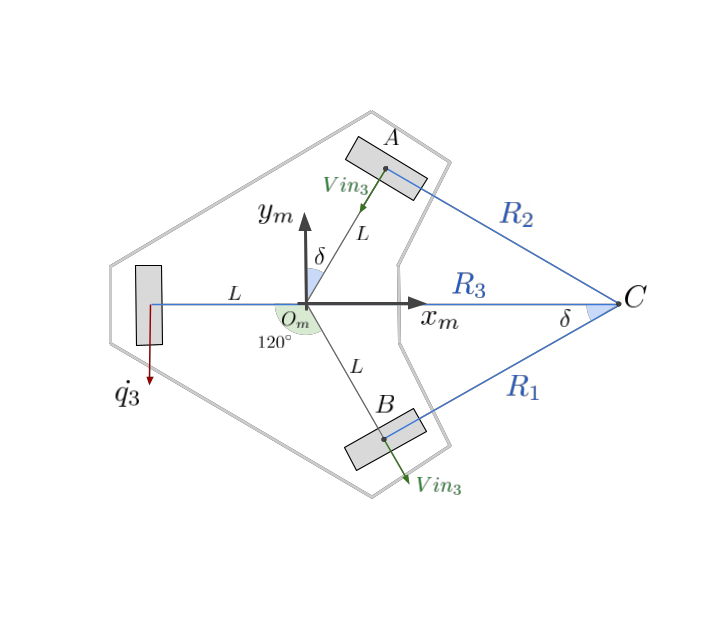
\includegraphics
        [width=0.4\textwidth]
        {figures/robot3.png}
    \caption{Induced velocity by the third wheel to the other ones}
    \label{fig:step1}
\end{figure}
Assuming that only the third wheel rotates with a velocity $\dot{q_{3}}$ and the other two wheels are inactive, we define as induced velocity $Vin_3$ the velocity that the first and second wheel gain from the third wheel. Using as reference Fig.\ref{fig:step1}, the robot turns around point $C$ with an angular velocity $\omega$ that can be expressed in two equivalent ways:
\begin{equation}
    \omega_3 = \frac{\dot{q_{3}}}{R_{3}} = \frac{V_{in3}}{R_{1}}         
    \label{omega}
\end{equation}
$R_3$ and $R_1$ can be easily computed from $\widehat{OBC}$ triangle:
\begin{equation*}
    R_3 = L + \overline{OC} = L + 2L = 3L         
\end{equation*}
\begin{equation*}
    R_1 = \frac{sin(\pi/2-\delta)}{sin(\delta)}L = \frac{cos(\delta)}{sin(\delta)}L 
\end{equation*}
Then from (\ref{omega}) we can express $Vin_3$ in terms of $\dot{q_3}$:
\begin{equation*}
    Vin_3 = \frac{R_1}{R_3}\dot{q_3}         
\end{equation*}

Due to the symmetrical mounting of the wheels, we can extend the previous result to a generic wheel $i$:

\begin{equation*}
    Vin_i = \frac{1}{3}\frac{cos(\delta)}{sin(\delta)}\dot{q_i}         
\end{equation*}

\subsubsection{Kinematic model in robot reference frame}
In the general case we have all the three wheels rotating with a specific velocity $\dot{q_{i}}$ and inducing a velocity $Vin_i$ to the others. We define a local frame $RF_i = [O_i, X_i, Y_i]$ for each wheel, $O_i$ is placed at the wheel's center, $Y_i$ is parallel to $\dot{q_i}$ and $X_i$ is placed in order to make $RF_i$ coherent with the direction of the z-axis of $RF_m$, see Fig. \ref{fig:step2}. 

\begin{figure}[h]
    \centering
    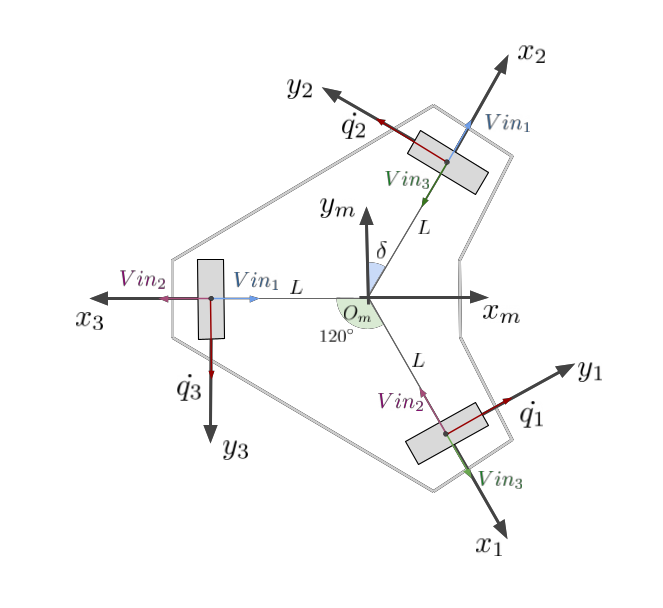
\includegraphics
        [width=0.4\textwidth]
        {figures/robot4.png}
    \caption{Resulting velocities w.r.t. $RF_i$}
    \label{fig:step2}
\end{figure}

The resulting velocities of each wheel $i$ w.r.t to $RF_i$ are the following:
\begin{gather}
    ^1V_1 =
    \begin{pmatrix} 
        Vin_3-Vin_2 \\
        \dot{q_{1}}
    \end{pmatrix}
    \\
    ^2V_2 =
    \begin{pmatrix} 
        Vin_1-Vin_3 \\
        \dot{q_{2}}
    \end{pmatrix}
    \\
    ^3V_3 =
    \begin{pmatrix} 
        Vin_2-Vin_1 \\
        \dot{q_{3}}
    \end{pmatrix}
\end{gather}
We can rewrite each of them w.r.t. $RF_m$ using:
\begin{equation*}
    ^mV_1 =\, ^mR_1\,^1V_1, \quad ^mV_2 =\, ^mR_2\, ^2V_2,\quad  ^mV_3 =\, ^mR_3\,  ^3V_3
\end{equation*}
Where:
\begin{equation*}
    ^mR_1 = R_{z}\left(-\frac{\pi}{2}+\delta\right), \, ^mR_2 = R_{z}\left(\frac{\pi}{2}-\delta\right), \, ^mR_3 = R_{z}\left(\pi\right)
\end{equation*}
\begin{equation*}
    R_{z}(\alpha) = \begin{pmatrix}
                \cos(\alpha) & -\sin(\alpha)\\
                \sin(\alpha) & \cos(\alpha)
            \end{pmatrix}
\end{equation*}

The whole angular velocity of the robot can be obtained by summing each single contribution $\omega_i$ (\ref{omega}):
\begin{equation*}
    \omega = \omega_1 + \omega_2 + \omega_3 
\end{equation*}
Therefore, the kinematic model w.r.t. the $RF_{m}$ is given by:
\begin{equation}
    \left\{
        \begin{array}{ll}
            \begin{pmatrix} 
                \dot{^m x_r} \\ 
                ^m y_r  
            \end{pmatrix} 
            = \frac
                {^m V_1 + ^m V_2 + ^m V_3}
                {3}\\
            
            \omega = \frac{1}{3L}\left(\dot{q_{1}} + \dot{q_{2}} + \dot{q_{3}}\right)
        \end{array}
    \right.
    \label{robot_ref}
\end{equation}

\subsubsection{Model in the world coordinate system}
Finally, starting from (\ref{robot_ref}), we can compute the kinematic model w.r.t to the world reference frame $RF_w$. The angular velocity remains the same, for the position we use a rotation around z-axis:

\begin{equation}
	\label{world_ref}
	\left\{
		\begin{array}{ll}
			\dot{^w x_r} = R_z(\theta)\, \dot{^m x_r}\\
			\dot{^w y_r} = R_z(\theta)\, \dot{^m y_r}\\
            \dot{\theta} = \omega
		\end{array}
	\right.
\end{equation}

Carrying out the calculations with $\delta=30^{\circ}$, from (\ref{world_ref}) we obtain (\ref{eq:kin_model}). \footnote{Matlab notebook \textit{proof\_model.mlx} in code folder shows the computation}
